%%%%%%%%%%%%%%%%%%%%%%%%%%%%%%%%%%%%%%%%%
% Beamer Presentation
% LaTeX Template
% Version 1.0 (10/11/12)
%
% This template has been downloaded from:
% http://www.LaTeXTemplates.com
%
% License:
% CC BY-NC-SA 3.0 (http://creativecommons.org/licenses/by-nc-sa/3.0/)
%
%%%%%%%%%%%%%%%%%%%%%%%%%%%%%%%%%%%%%%%%%
\documentclass{beamer}

%-------------------------------------------------------------------------------
%    PACKAGES AND THEMES
%-------------------------------------------------------------------------------
\mode<presentation> {

% The Beamer class comes with a number of default slide themes
% which change the colors and layouts of slides. Below this is a list
% of all the themes, uncomment each in turn to see what they look like.

%\usetheme{default}
%\usetheme{AnnArbor}
%\usetheme{Antibes}
%\usetheme{Bergen}
%\usetheme{Berkeley}
\usetheme{Berlin}
%\usetheme{Boadilla}
%\usetheme{CambridgeUS}
%\usetheme{Copenhagen}
%\usetheme{Darmstadt}
%\usetheme{Dresden}
%\usetheme{Frankfurt}
%\usetheme{Goettingen}
%\usetheme{Hannover}
%\usetheme{Ilmenau}
%\usetheme{JuanLesPins}
%\usetheme{Luebeck}
%\usetheme{Madrid}
%\usetheme{Malmoe}
%\usetheme{Marburg}
%\usetheme{Montpellier}
%\usetheme{PaloAlto}
%\usetheme{Pittsburgh}
%\usetheme{Rochester}
%\usetheme{Singapore}
%\usetheme{Szeged}
%\usetheme{Warsaw}


% As well as themes, the Beamer class has a number of color themes
% for any slide theme. Uncomment each of these in turn to see how it
% changes the colors of your current slide theme.

%\usecolortheme{albatross}
%\usecolortheme{beaver}
%\usecolortheme{beetle}
%\usecolortheme{crane}
%\usecolortheme{dolphin}
%\usecolortheme{dove}
%\usecolortheme{fly}
%\usecolortheme{lily}
%\usecolortheme{orchid}
%\usecolortheme{rose}
%\usecolortheme{seagull}
%\usecolortheme{seahorse}
%\usecolortheme{whale}
%\usecolortheme{wolverine}

% To remove the footer line in all slides uncomment this line
%\setbeamertemplate{footline} 

% To replace the footer line in all slides with 
% a simple slide count uncomment this line
\setbeamertemplate{footline}[page number] 

% To remove the navigation symbols from the bottom of 
% all slides uncomment this line
\setbeamertemplate{navigation symbols}{} 
}

\newcommand{\inlineml}[1]{\lstinline[language=ML, basicstyle=\small]{#1}}
\usepackage{graphicx} % Allows including images
\usepackage{booktabs} % Allows the use of \toprule, \midrule and \bottomrule in tables
%\usepackage {tikz}
\usepackage{tkz-graph}
\GraphInit[vstyle = Shade]
\tikzset{
  LabelStyle/.style = { rectangle, rounded corners, draw,
                        minimum width = 2em, fill = yellow!50,
                        text = red, font = \bfseries },
  VertexStyle/.append style = { inner sep=5pt,
                                font = \normalsize\bfseries},
  EdgeStyle/.append style = {->, bend left} }
\usetikzlibrary {positioning}
%\usepackage {xcolor}
\definecolor {processblue}{cmyk}{0.96,0,0,0}


%SVG
\usepackage{svg}


%listings
\usepackage{listings}
\usepackage{color}

\definecolor{dkgreen}{rgb}{0,0.6,0}
\definecolor{gray}{rgb}{0.5,0.5,0.5}
\definecolor{mauve}{rgb}{0.58,0,0.82}

\lstset{frame=tb,
  language=Java,
  aboveskip=3mm,
  belowskip=3mm,
  showstringspaces=false,
  columns=flexible,
  basicstyle={\small\ttfamily},
  numbers=none,
  numberstyle=\tiny\color{gray},
  keywordstyle=\color{blue},
  commentstyle=\color{dkgreen},
  stringstyle=\color{mauve},
  breaklines=true,
  breakatwhitespace=true,
  tabsize=3
}




% SVG images
\usepackage{svg}
\usepackage{calc}

\usepackage{tikz-cd}

%-------------------------------------------------------------------------------
%    TITLE PAGE
%-------------------------------------------------------------------------------
% Your institution as it will appear on the bottom of 
% every slide, may be shorthand to save space
\title[Short title]{Term Project: Robot Factory}
\author{Victor Carrillo, Joseba Celaya, Luis Mata}
% Your institution as it will appear on the bottom of 
% every slide, may be shorthand to save space
% Your institution for the title page
\institute[UCM/UAM/UPM]{

\medskip
}
\date{\today} 
%-------------------------------------------------------------------------------
%    BEGIN DOCUMENT
%-------------------------------------------------------------------------------
\begin{document}

% Title page
\begin{frame}
\titlepage 
\end{frame}

% Overview frame
\begin{frame}
\frametitle{Overview} 
\tableofcontents 
\end{frame}

%-------------------------------------------------------------------------------
%    PRESENTATION SLIDES
%-------------------------------------------------------------------------------

\section{Introduction}

\begin{frame}[containsverbatim]{Intro}
\begin{figure}[htbp]
  \centering
  %%\def\svgscale{0.5}
  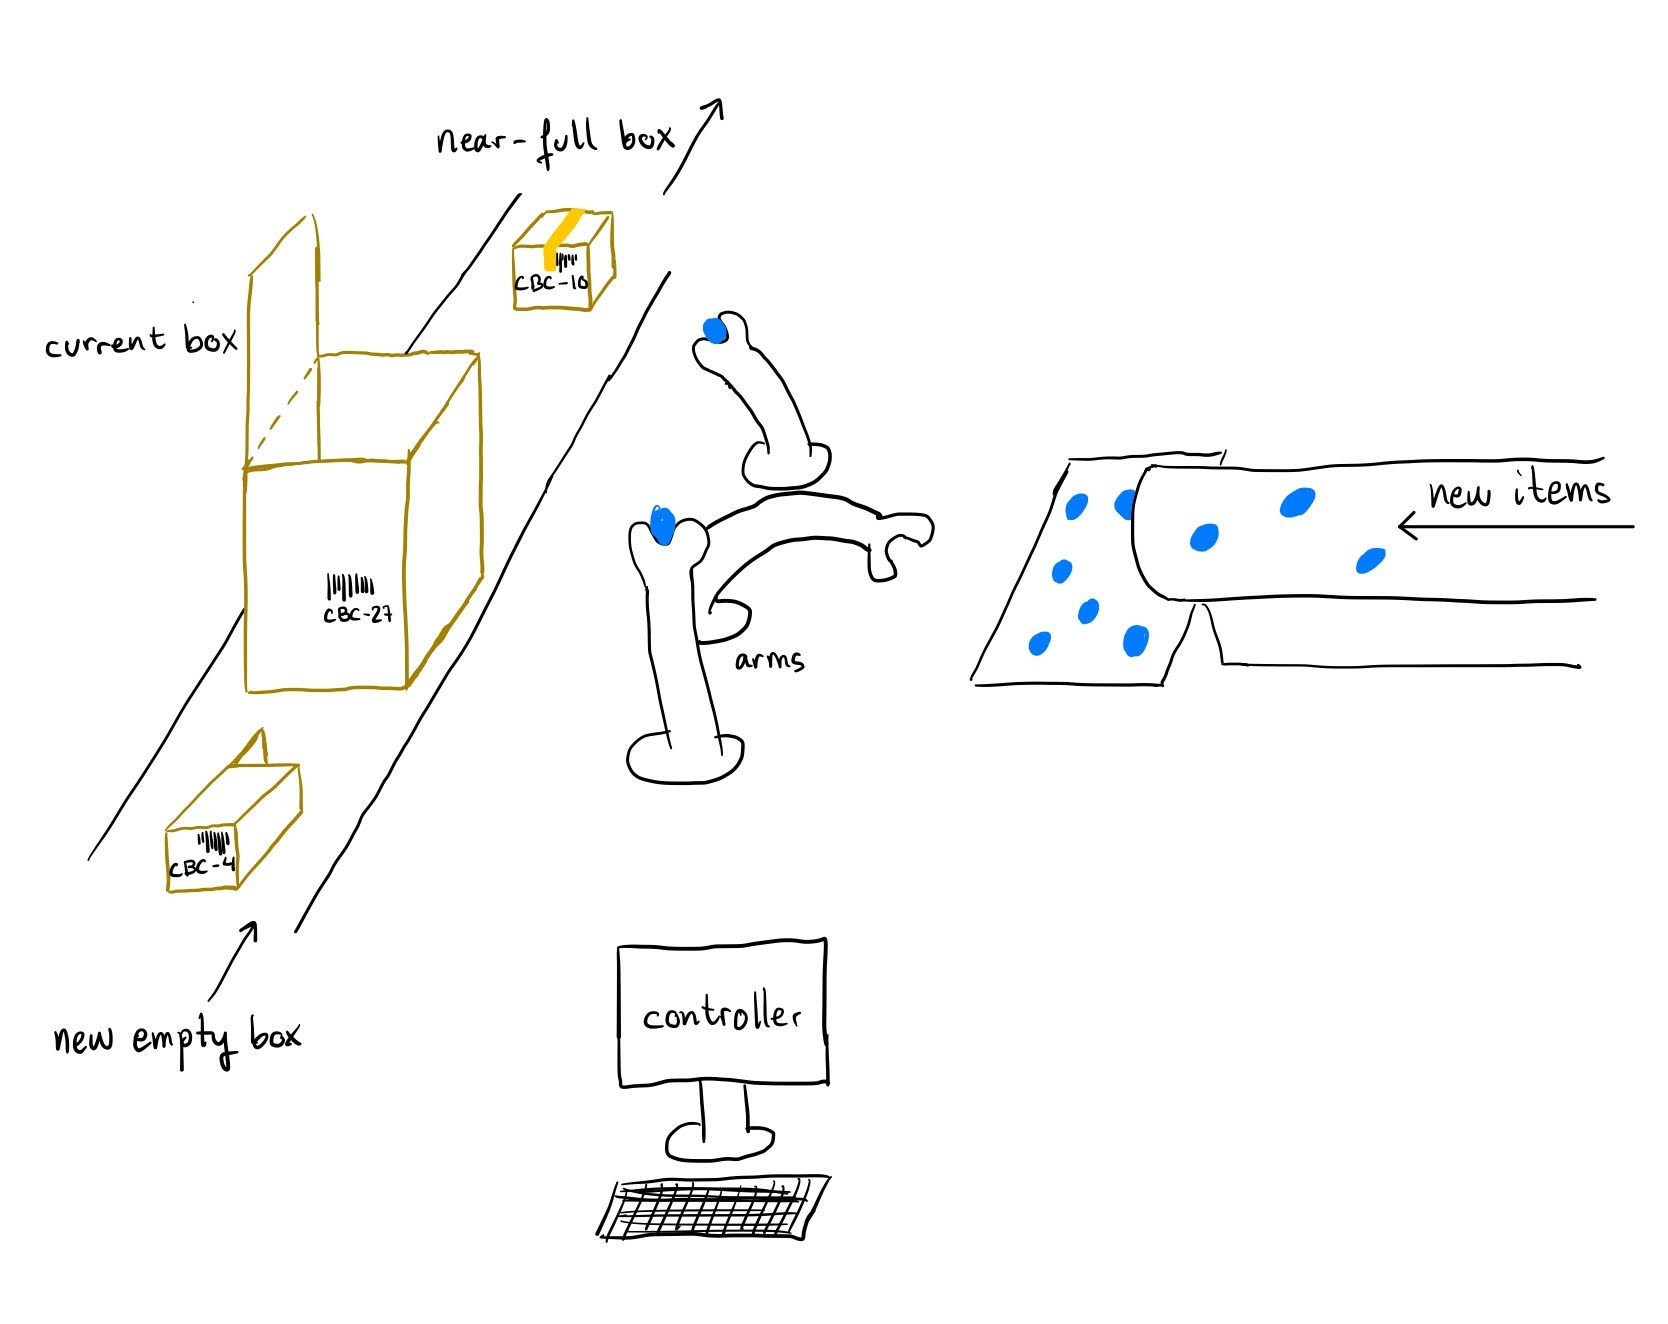
\includegraphics[scale=0.2]{figures/drawing.jpg}
\end{figure}
\end{frame}


\section{Model Variables and Events}

% Model 0 Sensors
\begin{frame}[containsverbatim]{Model 0 Variables}
\begin{figure}[htbp]
  \centering
  %%\def\svgscale{0.5}
  \includesvg[scale=1]{figures/map0.svg}
\end{figure}
\end{frame}


% Model 0
\begin{frame}[containsverbatim]{Model 0 Events}
\begin{figure}[htbp]
  \centering
  %%\def\svgscale{0.5}
  \includesvg[scale=1]{figures/model0.svg}
\end{figure}
\end{frame}


% Model 1 Sensors
\begin{frame}[containsverbatim]{Model 1 Variables}
\begin{figure}[htbp]
  \centering
  %%\def\svgscale{0.5}
  \includesvg[scale=0.12]{figures/map1.svg}
\end{figure}
\end{frame}


% Model 1
\begin{frame}[containsverbatim]{Model 1 Events}
\begin{figure}[htbp]
  \centering
  %%\def\svgscale{0.5}
  \includesvg[scale=1]{figures/model1.svg}
\end{figure}
\end{frame}


% Model 2 Sensors
\begin{frame}[containsverbatim]{Model 2 Variables}
\begin{figure}[htbp]
  \centering
  %%\def\svgscale{0.5}
  \includesvg[scale=0.12]{figures/map2.svg}
\end{figure}
\end{frame}


% Model 2
\begin{frame}[containsverbatim]{Model 2 Events}
\begin{figure}[htbp]
  \centering
  %%\def\svgscale{0.5}
  \includesvg[scale=0.08]{figures/model2.svg}
\end{figure}
\end{frame}


% Model 3 Sensors
\begin{frame}[containsverbatim]{Model 2B Variables}
\begin{figure}[htbp]
  \centering
  %%\def\svgscale{0.5}
  \includesvg[scale=0.12]{figures/map3.svg}
\end{figure}
\end{frame}


% Model 3
\begin{frame}[containsverbatim]{Model 2B Events}
\begin{figure}[htbp]
  \centering
  %%\def\svgscale{0.5}
  \includesvg[scale=0.8]{figures/model3.svg}
\end{figure}
\end{frame}


\section{Model Checking}

% Animation 0
\begin{frame}[containsverbatim]{Model Checking: 0 INITIALISATION}
\begin{figure}[htbp]
  \centering
  %%\def\svgscale{0.5}
  \includesvg[scale=0.08]{figures/models-animation0.svg}
\end{figure}
\end{frame}


% Animation 1
\begin{frame}[containsverbatim]{Model Checking: 1 PICK\_ITEM}
\begin{figure}[htbp]
  \centering
  %%\def\svgscale{0.5}
  \includesvg[scale=0.08]{figures/models-animation1.svg}
\end{figure}
\end{frame}


% Animation 2
\begin{frame}[containsverbatim]{Model Checking: 2 BOX\_ARR\_PHY}
\begin{figure}[htbp]
  \centering
  %%\def\svgscale{0.5}
  \includesvg[scale=0.08]{figures/models-animation2.svg}
\end{figure}
\end{frame}


% Animation 3
\begin{frame}[containsverbatim]{Model Checking: 3 BOX\_ARR}
\begin{figure}[htbp]
  \centering
  %%\def\svgscale{0.5}
  \includesvg[scale=0.8]{figures/models-animation3.svg}
\end{figure}
\end{frame}


% Animation 4
\begin{frame}[containsverbatim]{Model Checking: 4 SIGNAL\_ARM}
\begin{figure}[htbp]
  \centering
  %%\def\svgscale{0.5}
  \includesvg[scale=0.08]{figures/models-animation4.svg}
\end{figure}
\end{frame}


% Animation 5
\begin{frame}[containsverbatim]{Model Checking: 5 MOVE\_ARM\_PHY}
\begin{figure}[htbp]
  \centering
  %%\def\svgscale{0.5}
  \includesvg[scale=0.08]{figures/models-animation5.svg}
\end{figure}
\end{frame}


% Animation 6
\begin{frame}[containsverbatim]{Model Checking: 6 ARM\_BOX\_ARR}
\begin{figure}[htbp]
  \centering
  %%\def\svgscale{0.5}
  \includesvg[scale=0.08]{figures/models-animation6.svg}
\end{figure}
\end{frame}


% Animation 7
\begin{frame}[containsverbatim]{Model Checking: 7 PLACE\_ITEM}
\begin{figure}[htbp]
  \centering
  %%\def\svgscale{0.5}
  \includesvg[scale=0.08]{figures/models-animation7.svg}
\end{figure}
\end{frame}


% Animation 8
\begin{frame}[containsverbatim]{Model Checking: 8 RESTORE\_ARM\_PHY}
\begin{figure}[htbp]
  \centering
  %%\def\svgscale{0.5}
  \includesvg[scale=0.08]{figures/models-animation8.svg}
\end{figure}
\end{frame}


% Animation 9
\begin{frame}[containsverbatim]{Model Checking: 9 RESTORE\_ARM\_CTRL}
\begin{figure}[htbp]
  \centering
  %%\def\svgscale{0.5}
  \includesvg[scale=0.08]{figures/models-animation9.svg}
\end{figure}
\end{frame}


\end{document}